

%\documentclass[10pt,iop]{emulateapj}
\documentclass[preprint]{aastex}

\usepackage{url}
\usepackage{multirow}
\usepackage{amsmath}
\usepackage{xcolor}
%\citestyle{aa}

%\bibliographystyle{apj_w_etal}

\newcommand{\etal}{{et al.\/}}
\newcommand{\Prob}{\mathtt{P}}
\newcommand{\logL}{\log\mathcal{L}}
\newcommand{\unit}[1]{\footnotesize #1}
\newcommand{\PAPER}{\mathrm{PAPER}}
\bibliographystyle{apj_w_etal}

\newcommand{\Nconf}{31}
\newcommand{\Nsrc}{32}
\definecolor{orange}{RGB}{255,127,0}

	% End definitions

%\slugcomment{DRAFT: \today}

\shorttitle{EoR time}
\shortauthors{Jacobs et al.}

\begin{document}


\title{The PAPER-32 power spectrum measured at several redshifts}
\author{
Daniel C. Jacobs\altaffilmark{1},
Aaron R. Parsons\altaffilmark{2,8},
James E. Aguirre\altaffilmark{3},
Zaki Ali\altaffilmark{2},
Judd Bowman\altaffilmark{1},
Richard F. Bradley\altaffilmark{4,5,6},
Chris L.  Carilli\altaffilmark{7},
David R. DeBoer\altaffilmark{8},
Matthew R. Dexter\altaffilmark{8},
Nicole E. Gugliucci\altaffilmark{5},
Pat Klima\altaffilmark{5},
Dave H. E. MacMahon\altaffilmark{8}
Jason R. Manley\altaffilmark{9},
David F. Moore\altaffilmark{3},
Jonathan C. Pober\altaffilmark{2},
Irina I. Stefan\altaffilmark{10},
William P. Walbrugh\altaffilmark{9}}

\altaffiltext{1}{School of Earth and Space Exploration, Arizona State U., Tempe, AZ}
\altaffiltext{2}{Astronomy Dept., U. California, Berkeley, CA}
\altaffiltext{3}{Dept. of Physics and Astronomy, U. Pennsylvania, Philadelphia, PA}
\altaffiltext{4}{Dept. of Electrical and Computer Engineering, U. Virginia, Charlottesville, VA}
\altaffiltext{5}{National Radio Astronomy Obs., Charlottesville, VA}
\altaffiltext{6}{Dept. of Astronomy, U. Virginia, Charlottesville, VA}
\altaffiltext{7}{National Radio Astronomy Obs., Socorro, NM}
\altaffiltext{8}{Radio Astronomy Lab., U. California, Berkeley, CA}
\altaffiltext{9}{Square Kilometer Array, South Africa Project, Cape Town, South Africa}
\altaffiltext{10}{Cavendish Lab., Cambridge, UK}

\begin{abstract}
We present new observations from the Donald C. Backer Precision Array for Probing the Epoch of Reionization telescope which probe the redshift range of $6<z<9$, extending previously published single redshift results to cover the full range accessible to the instrument.  The removal of foregrounds depends heavily on the spectral smoothness of both instrumental response and foregrounds.  These spectra demonstrate a robust foreground removal of foreground signals to the thermal noise limit, leaving systematics on the scale of the noise. We find that these residual systematics are present throughout the observed frequency band are most likely some mixture residual foregrounds and instrumental systematics.
\end{abstract}

\keywords{reionization}


\section{Introduction}
The Epoch of Reionization (EoR), when the first stars ionized the pervasive cosmological Hydrogen in the last global phase change, is predicted to be observable in highly redshifted 21 cm radiation.  The Donald C. Backer Precision Array for Probing the Epoch of Reionization (PAPER, XXX)\footnote{\url{http:\\eor.berkeley.edu}} is a low frequency radio interferometer experiment dedicated to opening this window on the universe.  Challenges include foregrounds which are brighter by several orders of magnitude and limited collecting areas of first generation instruments which necessitate long integration times. Direct observation of hydrogen before and during re-ionization is predicted to deliver a wealth of cosmological and astrophysical data, including the nature of the first stellar objects and the timing and rate of galaxy formation, reviews on the physics of reionization as well as theory about the nature of foregrounds maybe be found in \citet{Furlanetto:2006p2267,Morales:2010p8093,Pritchard:2012p9555}.
Telescopes seeking to measure this signal include the Giant Metre-wave Radio Telescope (GMRT; \cite{Paciga:2013p9943}), the Low Frequency Array (LOFAR; \cite{Yatawatta:2013p9699}) and the Murchison Widefield Array (MWA; \cite{Bowman:2013p9950} and \cite{Tingay:2013p9022}). PAPER is located in the Karoo desert at the Square Kilometer Array-South Africa cite. PAPER has doubled in size on a yearly basis since 2009, making  EoR observations with each array.  Here we report on deep integrations made with a 32 element array in 2011, first described in \cite{Parsons:2013p9876}, hereafter P14.  In that work we described in detail a method used to estimate power spectra in the presence of bright foregrounds. Using this method we combined 120 XXX of data to place upper limits on the power spectrum of EoR. Here we extend this analysis of the same data include multiple redshift bins allowing us to place constraints on the time history of reionization.

This paper summarizes the observations and reduction methodology in \ref{sec:obs_meth}, present the new upper limits in \ref{sec:results}. In \ref{sec:models} we examine the impacts of the new data points on theory and conclude in \ref{sec:conclusion}.



%
%This signal is though to be the richest data set on the sky!  Many telescopes are searching for the power spectral signature of 
%HI.  Coarsely, models of 21cm emission can be distilled into two parameters. The redshift at which point the universe was 50\% ionized ($z_i$) and the transition time from mostly neutral to mostly ionized $dz$. Thus full coverage of the spectrum is essential.


%This paper extends the result ARP2013a to cover the redshift range XXX.

\section{Observations and reduction}
As the observations and methods in use are unchanged from those described in P14, we will offer a quick summary and refer the reader to \cite{Parsons:2013p9876} for a more in depth discussion.  A general overview of the PAPER system can be found in \cite{Parsons:2010p6757}, calibration of the primary beam in \cite{Pober:2012p8800}, and imaging results in \cite{Jacobs:2011p8438,Jacobs:2013p10014,Stefan:2013p9926}.  Sensitivity analysis described in \cite{Parsons:2012p9028} revealed that for the low gain elements employed by PAPER, a highly redundant ``grid'' type arrangement offers a significant sensitivity boost.  Each baseline samples a different mode of the EoR power spectrum. Each redundant baseline one samples a cosmological mode at high SNR before being combined with other different $k$ modes.  The PAPER South Africa 32 antenna deployment (PSA32) was arranged in a 4x8 grid.  Here we include only the three shortest types of spacings, those between adjacent columns within at least one row of each other, a selection containing 70 30m baselines.

Observations spanning the band between 100 to 200-MHz ($13.1>z>6.1$) were recorded at a resolution of 48kHz into 10.7s bins beginning Dec 7, 2011 and ending XXX for a total of XXX nights.  WIthin this set we included observations in the LST range 1h30m - 6h30m where the sky dominated system temperature is at a minimum.  


\section{Reduction}
Here we summarize our data reduction steps, for detailed descriptions see P14.

In several stages throughout the analysis process we take a 2D Fourier transform of the visibility spectra $V(t,\nu)$ into ``delay'/fringe rate' space.  In this space, smooth spectrum sources are physically localized to delays shorter than the light travel time length of the baseline (e.g. sources at the horizon, in the direction of the baseline vector) and fringe rates shorter than the sidereal rate.  In the Fourier space sources are highly localized but are convolved with the dual of the spectrum sampling function, which is uneven due to flagging of interference.  To account for this missing data we use a CLEAN like, iterative, peak finder and subtraction algorithm which is limited to finding peaks within the physically allowable ranges, and occasionally beyond, where necessary to account for spectral and temporal dispersion. 

The data analysis pipeline essentially consists of iterative application of the delay/fringe rate transform process, with an ever tightening CLEAN box, interleaved with stages of averaging (time, night, and baseline), before finally computing a power spectrum.  This final step takes advantage of the redundant baselines to make an unbiased power spectrum estimate by cross-multiplying identical baselines.  


\subsection{Initial Averaging}
  First, the raw data are down-selected to just the 30m long baselines. %I know this isn't technically true, but I think its important that the downselect is obvious.
   The visibilities are then compressed in the frequency and time directions by filtering delay modes above the horizon and highest frequency fringe rates for a 300m baseline.  This filtering is done in tandem with a radio frequency interference (RFI) flagging step, using the CLEAN residuals to flag 4$\sigma$ RFI in the absence of bright sky signals and then feeding the flags back into another iteration of the compression step. This mitigate the effects of RFI leaking around the filter to generate a cleaner averaged data set and results in a time and frequency bin of length 45.7s and width 400kHz. % XXX check  
  This process reduces the data volume by a factor of \~40.
  
\subsection{Calibration}
We model per-antenna complex gains with a phase slope and spectral amplitude.  Because the array samples correlations redundantly, the relative calibration between antennae is numerically overdetirmined and tractable as a linear algebra problem.  These solutions vary little over the observing period and exhibit less than 1\% rms variation. %XXX is that so??? 

By itself, the redundant solution is completely independent of any sky model. The redundant solution contains two free delay parameters and an overall amplitude scale. We fit the two delay parameters to a model of Pictor A, Fornax A, and the Crab Nebula during a time when the sky is dominated by these three sources while marginalizing over the unknown ratio between the three sources. With the delays in place we are now able form a beam on Pictor A and (for each channel) set the overall amplitude to the calibration value found in \cite{jacobs:2013b}.
  
%The success of the remainder of the processing stages hinges on the spectral stability of the data, which can easily be assessed by comparing redundant baselines. In figure XXX we see the rms of the ratios between redundant calibrations, before and after the calibration has been applied.  
\begin{figure}
\centering
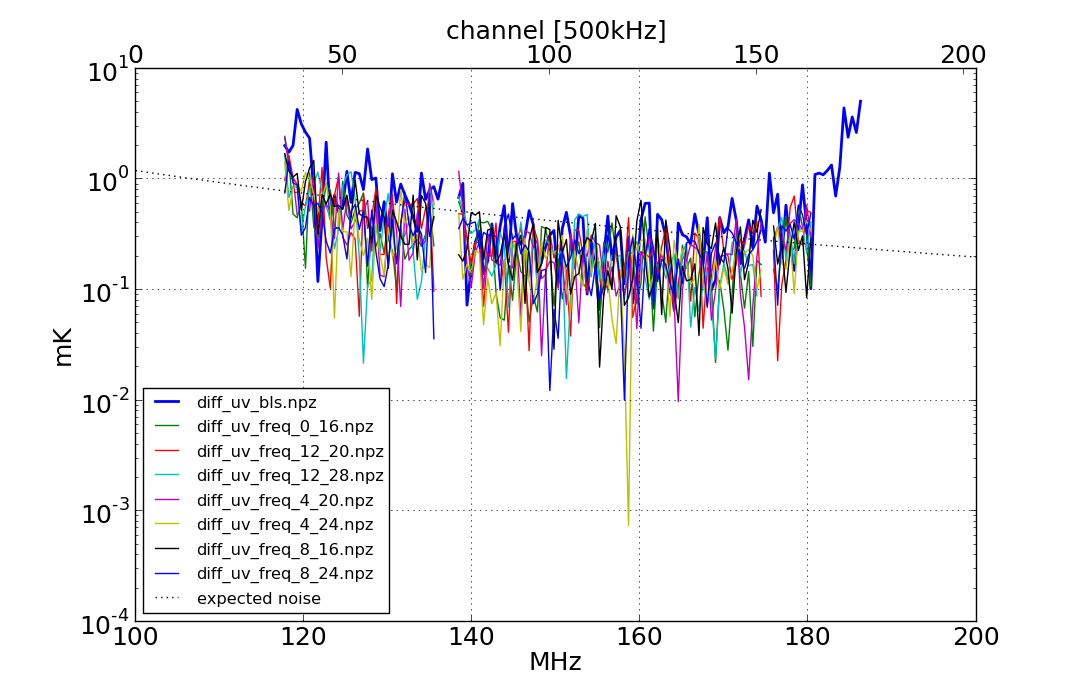
\includegraphics[width=\textwidth]{figures/trms_by_baseline.png}
\caption{\label{fig:noise} The residual noise after filtering foregrounds is consistent with the theoretical noise (dotted line).  Here we estimate residual noise by differencing spectral channels and redundant baselines. The noise spectrum is characterized by an overall slope towards lower frequencies owing to the power law slope of the galactic spectrum which drives the system temperature.  At both high and low edges the noise is also driven up by the use of a hamming window in the foreground filter. Less is known about foregrounds at the edges of the band which drives up the residuals.}
\end{figure}
%XXX more, and a plot of those redundancy residuals
\subsection{Foregrounds}
Foregrounds are filtered from the calibrated data by removing all bright delay components with light travel times less then the baseline length. Where during the previous compression step a  horizon of 300m (1800ns)  was used to calculate the window size we now choose a window corresponding to the 30m baselines under study.  At this point a four hour long running mean is subtracted. This removes excess correlation due to cross-talk in the analog signal chain. The residuals are then flagged once more for RFI before the XXX nights of data are averaged into 10 minute long local sidereal time (LST) bins.  During averaging we found that some lst bins were dominated by very bright data points due to some non-noise-like data points. As these were very rare we found that removing the ten brightest points from every bin, a small median filter, was quite effective.   The root mean square of the residual signal (seen in Figure \ref{fig:noise}) at the end of this process is close to the 1mK level expected given the total integration time.

%This step is the first point at which signal loss could occur. To measure the loss we add white noise into the data at a level sufficient to double the system temperature (to make it easily detectable on the output), subtract  and then measure the fractional difference post filtration. We recover XXX\% of the injected signal.

%delay transform, covariance projection (lossless, and lossy), bin and bootstrap average,
\subsection{Power Spectrum}
\begin{figure}
\centering
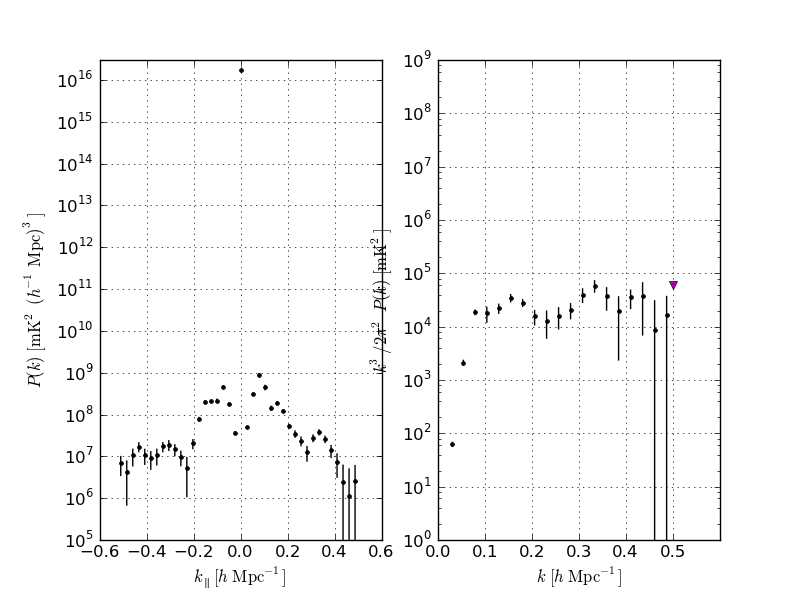
\includegraphics[width=0.45\textwidth]{figures/pspec_Mar24_psa32_zbins_1_80_119_I.png}
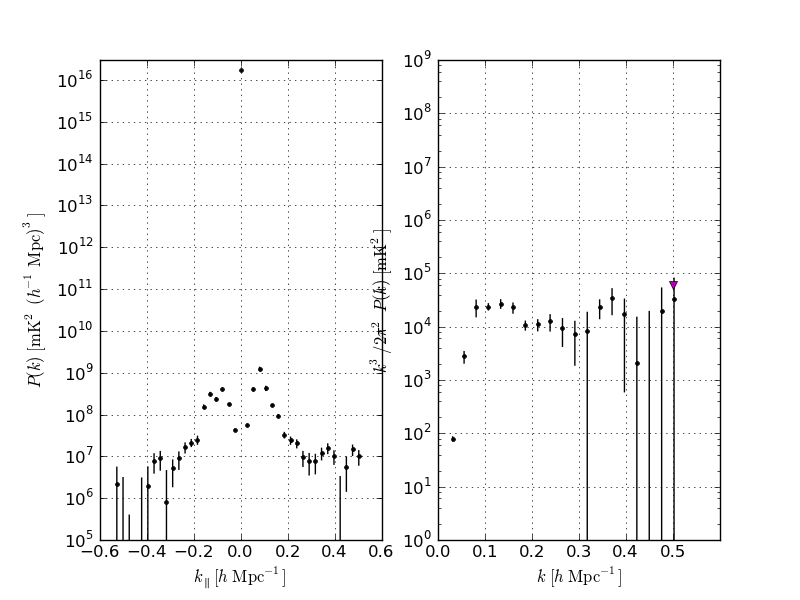
\includegraphics[width=0.45\textwidth]{figures/pspec_Mar24_psa32_zbins_1_100_139_I.png}
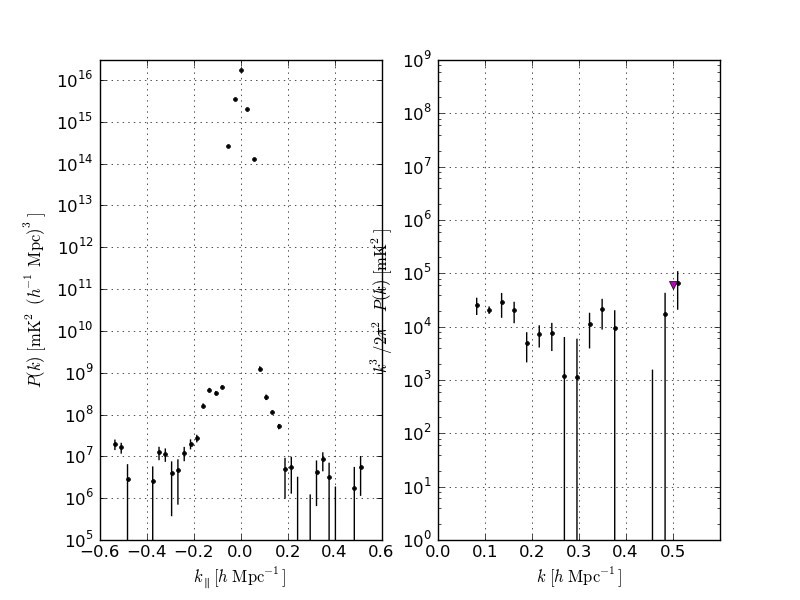
\includegraphics[width=0.45\textwidth]{figures/pspec_Mar24_psa32_zbins_1_110_149_I.png}
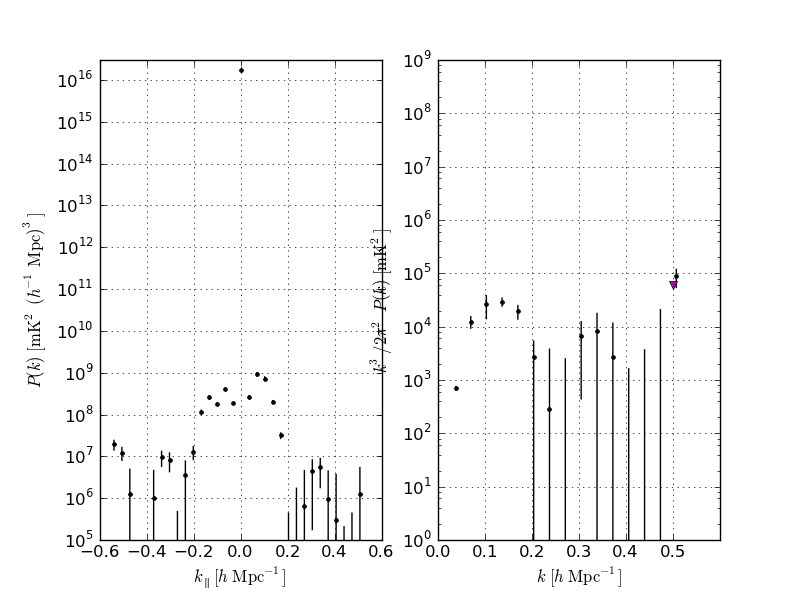
\includegraphics[width=0.45\textwidth]{figures/pspec_Mar24_psa32_zbins_1_119_150_I.png}
\caption{\label{fig:pspecs} Clockwise from top left: power spectra centered on redshifts 8.5, 7.9, 7.6 and 7.5 (frequencies: 149.5, 159.5 164.5, and 167 MHz) at a bandwidth of 20MHz}
\end{figure}
\section{Discusion}

\begin{figure}
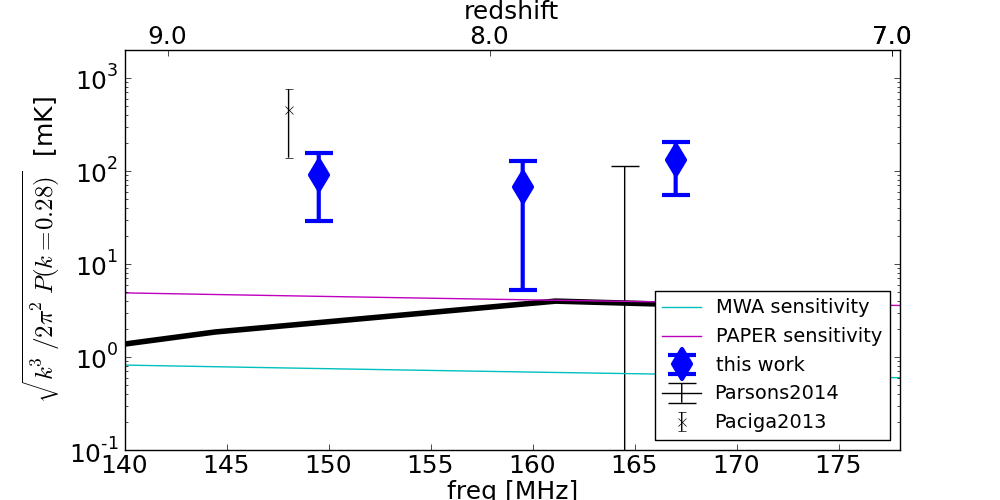
\includegraphics[width=\textwidth]{figures/psa_p3k_vs_z_28.png}
\caption{Power spectrum amplitude at k=0.28 hMpc$^-1$.  Paciga 2013 GMRT marked with an 'x', Parsons 2013 PAPER limit marked with thin black, this work marked with thick blue diamonds.}
\end{figure}

\section{Conclusions}

Here we have, using the same dataset extended the expanded the redshift coverage of \cite{Parsons:2013p9876} cover the range $10>z>7$.  These measurements demonstrate a precision removal of foregrounds to one part in ten million across the entire redshift range of interest. Though, with only 32 antenna, this data lacks the sensitivity to exclude all but the most extreme models, it does demonstrate the ability of the wideband filtration method to affectively remove foregrounds to the precision needed to integrate XXX nights to the thermal noise limit.  As future observations with PAPER  will add sensitivity primarily by increasing to 128 antennae this projects well for our ability to reach design sensitivity. 

%\begin{align}
%\label{eq:BrightnessFluctuations}
% \Delta T &\approx \frac{T_S - T_{CMB}}{1 +z} \tau_{21} \nonumber\\
% &\approx T_0(z) \left( \frac{T_S - T_{CMB}}{T_S} \right) x_{HI} (1 + \delta) 
%\end{align}
%where $T_S$ is the 21cm line spin temperature, $x_{HI}$ is the local ionization fraction and $\delta$ is the mass over-density. All, save $T_0$, are position dependent.  $T_0$ encodes the global temperature evolution due to cosmological expansion
%\begin{align}
% T_0(z) & = 23~{\rm mK}~\left( \frac{\Omega_b h^2}{0.02} \right) \left[ \left(
% \frac{0.15}{\Omega_m h^2} \right) \left( \frac{1+z}{10} \right) \right]^{1/2}\nonumber\\
% & = 25~{\rm mK}~\left( \frac{1+z}{10} \right)^{1/2}
%\label{eq:Prefactor}
%\end{align}
%\citep[see, e.g., ][]{zaldarriaga_et_al2004,furlanetto_et_al2006}, where we have used the
%Planck 2013 parameters \citep{planck_et_al2013}.  



\bibliography{library}

\end{document}
